% Implications, Not Just Words -- draft for arXiv (cs.CL / cs.AI). Every figure in this document comes from evals/REPORT.md
% (rebuilt from the saved answers by `python -m evals.report`); change the numbers there, never here by hand.
\documentclass[10pt,twocolumn]{article}
\usepackage[margin=0.75in,columnsep=0.25in]{geometry}
\usepackage[T1]{fontenc}
\usepackage[utf8]{inputenc}
\usepackage{times}
\usepackage{microtype}
\usepackage{amsmath}
\usepackage{booktabs}
\usepackage{graphicx}
\usepackage{xcolor}
\usepackage{tikz}
\usetikzlibrary{arrows.meta,positioning}
\usepackage[round,authoryear]{natbib}
\usepackage[hidelinks]{hyperref}
\usepackage{enumitem}
\setlist{nosep,leftmargin=*}

\title{Implications, Not Just Words: Label Engineering for a Small Local Language Model\\Writing Fitness Coaching Messages}
\author{Guillermo Alfonso Medrano Sanchez\\Independent researcher\\\texttt{gcapitalgt@gmail.com}}
\date{}

\begin{document}
\maketitle

\begin{abstract}
Small language models that run on consumer hardware allow personal coaching without sending health data to a hosted
service, but given numeric summaries they misread comparisons, attach the wrong implications to them and copy the
structure of their instructions. We study \emph{label engineering}: code turns every number a message depends on into
a verbal verdict, states what each verdict implies for the user's goal, orders the priorities and fixes the answer
plan, so that the model only writes the sentences. In a deployed fitness assistant running qwen3:8b (4-bit) on an
8\,GB GPU, we compare eight representations of a weekly review and up to seven designs for each of two daily messages,
on 30 synthetic cases per message type (20 for tuning, 10 held out), scored by a frozen checklist whose precision we
check by reading its flags. On held-out weeks the share of answers passing every check rose from 3\% to 87\%
(Wilcoxon $p=0.002$), at 5.2\,s per review against 39.6\,s for the original thinking-mode prompt. The advice became
correct only when code supplied the implications, priorities and plan; adding the figures back to that design kept the
advice correct but brought invented figures back (63\% of answers passing every check). The approach transferred to checkpoint comments (33\% to 100\%) and
morning briefings (37\% to 100\%), improved the pass rate on three other model families in eight of nine comparisons,
and on a conversational agent passed 90--92\% of answers on two fresh case sets against 15--21\%. A deployed message
that told a user to do squats ``to add steps'' exposed rules our checklist lacked. In a blind comparison by six people
the two designs were rated about even (56\% of decisive choices for words): ahead on the weekly review, behind on the
chat, with little agreement between raters. We report the failure modes that labels introduce and derive nine design
rules.
\end{abstract}

% ─────────────────────────────────────────────────────────────────────────────
\section{Introduction}
\label{sec:intro}

A personal fitness assistant handles data that users may not want to send to a hosted model. Running an 8B-parameter
model locally removes that dependency and exposes the limits of small models on a task that looks simple: turning a
week of tracked steps, calories, protein and workouts into a short, correct review with concrete recommendations.
CALVIS, a Telegram fitness assistant that runs entirely on a consumer PC, originally passed the model aggregates,
targets and status codes. Its outputs contained four kinds of error:
(i)~misread comparisons (``2650\,kcal, slightly below the 2000\,kcal target'');
(ii)~correct facts with the wrong implication, such as recommending more walking before any food change to a user
who under-ate;
(iii)~internal codes in user-facing text (``which is a status~3'');
(iv)~copies of the instruction structure: an instruction list ending in ``a brief workout or rest day note'' was
followed by ``Rest day is okay'' on training days.

We evaluate one remedy, \emph{label engineering}. Deterministic code computes everything the message depends on:
each comparison, its size, its consequence for the user's goal, the priority order, the kind of fix and the plan of
the answer. It passes these to the model as short sentences without digits. The model's role reduces to surface
realization, the final stage of the classic natural language generation (NLG) pipeline \citep{reiter2000building}.
Pipelines of this kind are established in data-to-text generation; what we add is a stepwise measurement, in a small,
4-bit quantized model deployed on consumer hardware, of which layer of verbalized information removes which class of
error, and of the errors that each layer introduces. We ask:
\begin{itemize}
\item[\textbf{RQ1}] Which layers of the representation (verbal verdicts, implications, priorities, answer structure)
change factual errors, the correctness of the advice and adherence to the format?
\item[\textbf{RQ2}] Do the gains transfer to other message types, what do labels break, and what do deterministic
answer checks with one redraft add once the representation is fixed?
\item[\textbf{RQ3}] Do the gains hold on other model families and on a conversational agent that answers free-form
questions, where the question, not a schedule, decides what the message must cover?
\item[\textbf{RQ4}] Do people who read both versions blind prefer the label design, and do they see the difference in
accuracy that the checklists measure?
\end{itemize}

\paragraph{Contributions.}
\begin{itemize}
\item A controlled sequence of eight representations of the same weekly data, from raw numbers to labels with
implications and a code-decided plan, evaluated on held-out cases (\S\ref{sec:res-weekly}). Verbal verdicts reduce
hallucination; the correctness of the advice changes only when code supplies the implications; format failures follow
the structure of the prompt.
\item A replication on two further messages with an ablation of answer checks (\S\ref{sec:res-messages}), including a
revision that improved the tuning set and degraded the held-out set.
\item Model-free measures of a representation, notably \emph{verdict coverage} (the share of decisions a message needs
that the prompt states explicitly) and a count of statements that are false as worded. These located defects in the
production prompts before any model was run (\S\ref{sec:res-rep}).
\item A replication on three further model families (\S\ref{sec:res-models}), including the one model on which the weekly
review could not meet its format under either representation, and a fourth surface, a conversational agent
(\S\ref{sec:res-chat}), evaluated on a sequence of fresh case sets each used once, with every post-hoc change disclosed.
\item A small blind human comparison (six raters, four message types, \S\ref{sec:res-human}) that does not support a
general preference for the label design, shows almost no agreement between raters, and shows that raters did not notice
the accuracy gain the checklists measure.
\item An evaluation protocol for small deployments: a frozen, self-contained checklist whose precision is measured by
reading its flags; version fingerprints so that only identical configurations are pooled; a tuning/held-out split
(\S\ref{sec:eval}).
\end{itemize}

% ─────────────────────────────────────────────────────────────────────────────
\section{Related Work}
\label{sec:related}

\paragraph{Numeracy in language models.} Language models represent and manipulate numbers unreliably
\citep{spithourakis2018numeracy,wallace2019numbers,thawani2021representing}. Arithmetic accuracy depends on the
surface form of numbers and on tokenization \citep{nogueira2021investigating,singh2024tokenization}, which has
motivated dedicated number encodings \citep{golkar2023xval}. We leave the model unchanged and remove numeric
reasoning from inference instead.

\paragraph{Data-to-text generation.} Pipeline NLG separates content determination and document planning from
realization \citep{reiter2000building,gatt2018survey}. End-to-end neural data-to-text systems hallucinate and omit
facts \citep{wiseman2017challenges}; explicit content selection and planning reduce both
\citep{puduppully2019data}. \citet{kasner2022neural} verbalize data items with templates and let pretrained models
fuse and rephrase them. Label engineering applies such a pipeline to prompting a general-purpose SLM: control is
exercised through the content of the prompt rather than through decoding constraints, and the document plan is itself
expressed in text.

\paragraph{Offloading computation to code.} Program-aided and tool-using models delegate arithmetic to an interpreter or a
calculator \citep{gao2023pal,schick2023toolformer}. There the model still decides what to compute and how to phrase it; in label
engineering the computation, the comparison and the plan are fixed in advance by code and the model receives only their verbal
result. We did not run a program-aided or tool-using baseline (Section~\ref{sec:limitations}).

\paragraph{Numbers as words for language models.} The closest work we found is \citet{caut2025wordalisations}, who generate
natural-language narratives from numerical data with LLMs through engineered prompt templates (``wordalisations'') and evaluate
them in three domains, with LLM and human judges. We differ in the target (short advice messages tied to a user's goal), in
the model (a 4-bit 8B model run locally), and in the measurement: a stepwise comparison of layers of verbalized information
on held-out cases, with the errors each layer introduces. Prompt formatting changes model behavior substantially
\citep{sclar2024quantifying}, which is consistent with, but does not explain, our findings. The term ``label engineering''
here means writing the verbal descriptions of the data; it is unrelated to the label words (verbalizers) of prompt-based
classification. \citet{arai2025evaluating} evaluate how well LLMs understand numerical time series when generating text
from them; we instead remove that step from the model, and test with an ablation (A9) what is left once the digits
are put back.

\paragraph{Language models for personal health.} Wearable data have been given to LLMs by fine-tuning on sensor summaries
\citep{cosentino2024personal}, by prompt enhancement for health prediction \citep{kim2024healthllm} and through agents that write
code to analyze them \citep{merrill2024transforming}. We use none of these: no fine-tuning, a local model, and deterministic
verbalization before the prompt.

\paragraph{Hallucination and context.} \citet{ji2023survey} survey hallucination in NLG. Irrelevant context degrades
LLM reasoning \citep{shi2023distracted}, and where information sits in a long context matters
\citep{liu2024lost}. We observe a generation-side counterpart: lines that the message does not need tend to be
verbalized.

\paragraph{Evaluation and correction.} Our checklist follows behavioral testing \citep{ribeiro2020checklist} and
verifiable instruction checks \citep{zhou2023ifeval}. Our answer checks give the model external, deterministic
feedback and one redraft, unlike self-refinement \citep{madaan2023selfrefine}; models struggle to correct their
reasoning without such feedback \citep{huang2024cannot}. We use an LLM judge only as a secondary signal, given the
known biases of LLM judges \citep{zheng2023judging}. Chain-of-thought prompting \citep{wei2022chain} and thinking
modes \citep{qwen3} trade latency for reasoning; we compare against one such configuration.

% ─────────────────────────────────────────────────────────────────────────────
\section{System, Task and Data}
\label{sec:system}

\paragraph{Messages.} Three messages are generated from tracked data.
The \emph{weekly review} has two paragraphs: observations about steps, calories, protein and workouts against the
user's targets, then one to three numbered, concrete recommendations. It takes two model calls (one per paragraph) in
every design except the original one.
The \emph{checkpoint comment} follows each of four daily checks (12:00, 15:00, 19:00, 23:59). It says how the block
that just closed went, where the day stands and what the carry-over leaves for the rest of the day, and it proposes
one action; the last check of the day is a two-to-three-sentence summary.
The \emph{morning briefing} has two model-written parts: a reflection on yesterday that opens with a greeting, and two
to three suggestions for today (food, movement, workout). Its original yesterday prompt already used verbal
classifications; its today prompt used figures.

\paragraph{Model.} qwen3:8b \citep{qwen3} in the Q4\_K\_M 4-bit format \citep{llamacpp}, served by Ollama
\citep{ollama} on an NVIDIA RTX~4060 (8\,GB), in non-thinking mode at temperature 0.1, except configuration A0,
which uses thinking mode.

\paragraph{Cases.} Thirty synthetic cases per message type, built through the production code's own functions so that
every design receives exactly what it would receive in production: the dictionary the analysis code assembles from
the database (weekly review), the block figures of the production deviation engine (checkpoint) and the inputs as
the production function formats them (briefing). Twenty \emph{tuning} cases cover situations where a small model
fails: a met target the model must not ask to increase, very large gaps, missing data, each training phase, nothing
logged, rain or unknown weather, disliked foods and every carry-over strategy. Ten \emph{held-out} cases were written
later as different situations and were not used to design any version, with one exception discussed in
\S\ref{sec:limitations}. The original prompts were extracted from the production code without modification; golden
files captured beforehand pin them byte for byte.

% ─────────────────────────────────────────────────────────────────────────────
\section{Label Engineering}
\label{sec:method}

Let $x$ be the numeric state of a message: targets, aggregates, slopes, schedule fractions, logged entries and
weather. A labeler $L$ is deterministic code that maps $x$ to a \emph{view} $v=L(x)$: a short text built from fixed
vocabularies that contains no digits, except the temperature, which the user asked to keep. The prompt is the identity
header, the view and the format rules. A view carries up to five layers:
\begin{enumerate}
\item \textbf{Verdicts}: each metric's position against its target, with a size word from a fixed scale (``about a
third over'') and the trend relative to the target.
\item \textbf{Implications}: what the verdict means in the current phase (fat loss, maintenance, muscle gain), e.g.\
``this eats into the planned deficit''.
\item \textbf{Priorities}: problems ordered by deviation $\times$ phase weight; in the checkpoint labeler for a
fat-loss phase, calories over plan weigh 1.5, protein behind 1.3, steps behind 1.0 and calories under 0.
\item \textbf{Fix kinds and constraints}: food, movement or training; what to leave unchanged; the only links between
metrics that follow from the verdicts.
\item \textbf{Plan}: what the answer must contain, stated as one sentence.
\end{enumerate}
Layer~1 combines two operations that we separate by ablation (\S\ref{sec:res-weekly}): removing the digits, and
stating verdicts that the numeric prompt left implicit.
Figure~\ref{fig:pipeline} shows the pipeline and Figure~\ref{fig:example} one week under three representations.

\begin{figure}[t]
\centering
\resizebox{\columnwidth}{!}{%
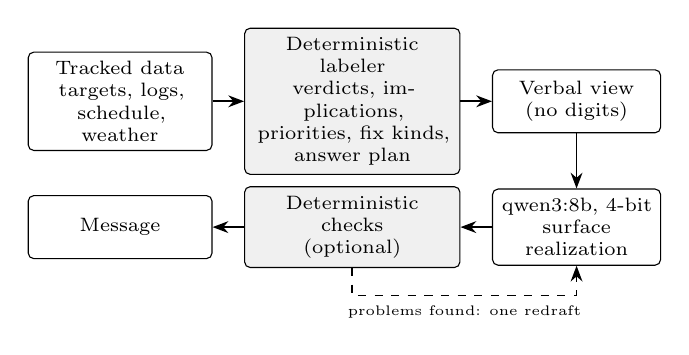
\begin{tikzpicture}[
  box/.style={draw, rounded corners=2pt, align=center, font=\scriptsize, minimum height=8mm, text width=#1},
  box/.default=21mm,
  arr/.style={-{Stealth[length=2mm]}, semithick}]
\node[box=21mm] (data) {Tracked data\\targets, logs,\\schedule, weather};
\node[box=25mm, right=4mm of data, fill=gray!12] (lab) {Deterministic labeler\\verdicts, implications,\\priorities, fix kinds,\\answer plan};
\node[box=19mm, right=4mm of lab] (view) {Verbal view\\(no digits)};
\node[box=19mm, below=7mm of view] (slm) {qwen3:8b, 4-bit\\surface\\realization};
\node[box=25mm, left=4mm of slm, fill=gray!12] (chk) {Deterministic checks\\(optional)};
\node[box=21mm, left=4mm of chk] (out) {Message};
\draw[arr] (data) -- (lab);
\draw[arr] (lab) -- (view);
\draw[arr] (view) -- (slm);
\draw[arr] (slm) -- (chk);
\draw[arr] (chk) -- (out);
\draw[arr, dashed] (chk.south) -- ++(0,-3.5mm) -| node[pos=0.25, below, font=\tiny] {problems found: one redraft} (slm.south);
\end{tikzpicture}}
\caption{Label engineering. Code performs content determination and document planning; the SLM performs surface
realization. Answer checks are optional and evaluated by ablation.}
\label{fig:pipeline}
\end{figure}

\begin{figure*}[t]
\centering\scriptsize
\begin{tabular}{@{}p{0.31\textwidth}p{0.30\textwidth}p{0.35\textwidth}@{}}
\toprule
\textbf{Numbers (A1)} & \textbf{Labels v1: verdicts (A2)} & \textbf{Labels v6, recommendations view (A7)}\\
\midrule
\ttfamily Goal phase: Fat Loss\newline
Targets: 10,000 steps, 2,000 kcal, 150g protein\newline
Peak step hour: 18:00 (avg 1450 steps)\newline
Stability (avg / CV\% / slope per day):\newline
\ Steps: avg 10200, CV 10.0\%, slope +15.0/day\newline
\ Calories: avg 2650 kcal, CV 14.0\%, slope +60.0 kcal/day\newline
\ Protein: avg 158 g, CV 8.0\%, slope +2.0 g/day\newline
Vs targets (precomputed, use as-is):\newline
\ Steps: 10200 vs 10,000 target (+200, target met)\newline
\ Protein: 158g vs 150g target (+8g, target met/exceeded)\newline
Workouts this week: 3/7\newline
Caloric goal hit (within +/-10 kcal): 1/7 days
&
\ttfamily Phase: Fat Loss\newline
Steps: right at the goal, just above it; holding steady through the week; fairly consistent from day to day.\newline
Calories: far over the target; rising quickly through the week; fairly consistent from day to day.\newline
Protein: right at the goal, just above it; rising gradually through the week; very consistent from day to day.\newline
Needs attention: calories (far over the target).\newline
On track: steps, protein.\newline
Workouts this week: a steady week, three sessions.
&
\ttfamily Main point: The main issue this week is calories (very large gap): this eats into the planned deficit, so
fat loss slows or stalls.\newline
What to work on, most important first:\newline
\ First: calories, miles over the target (about a third off). Why it matters: this eats into the planned deficit,
so fat loss slows or stalls. Kind of fix: food: trim portions or cut a snack, rather than adding exercise.\newline
Leave unchanged (make no recommendation about these): steps, protein.\newline
Plan: a habit for calories; a second, different habit for calories.\\
\midrule
\multicolumn{3}{@{}p{0.98\textwidth}@{}}{The numeric block states a verdict for steps and protein but not for
calories (verdict coverage 66\%). The model wrote ``2650\,kcal, slightly below the 2000\,kcal target''. Checkpoint
comment, case~01 at noon, numbers: \texttt{Calories: live 850 kcal vs expected 550 kcal (status 3, over target);
target next block -300 kcal (raw carry -300 kcal \textemdash{} user is 300 kcal over daily budget)}. With 850 of 2,200\,kcal
eaten, the last statement is false as worded. Labels: \texttt{Calories: in this block about half over this block's
share; the day so far is far over plan; the rest of the day has a fair bit less food to work with than usual. For
the goal: in a cut this eats into today's deficit.}}\\
\bottomrule
\end{tabular}
\caption{The same week (tuning case 07) as the model sees it under three representations, and one checkpoint line
under two. Excerpts; the full prompts are in the released code.}
\label{fig:example}
\end{figure*}

\paragraph{Weekly review versions.} Table~\ref{tab:attempts} lists the configurations. v1 holds layer~1; v2 adds gap
sizes, directions, a ``keep as is'' list and an advice goal; v3 adds layers 2--4; v4 presents v3 as one view per
question (observations; recommendations); v5 adds layer~5 as a list; v6 states the same plan as one sentence.

\paragraph{Checkpoint labels.} The block result is stated against the block's share and the day so far against the
cumulative plan. The carry-over is expressed as the rest of the day compared with a normal rest of the day (``a fair bit
less food to work with than usual''). The view adds implications, priorities and foods from the user's own list that
fit the need (lean protein: at least 8\,g protein and 5\,g per 100\,kcal; light: at most 200\,kcal; energy-dense: at
least 250\,kcal; disliked foods excluded), together with an outdoor verdict (not suitable at WMO weather code 51 or
above, or 0.5\,mm precipitation) and a plan. Version~2 removes from the day's last check every line that does not
describe the day (weather, outdoor verdict, foods, morning feedback) and asks to keep the size words as given.

\paragraph{Briefing labels.} Yesterday is stated as each result with a size word, its implication and the link to
today's changed target (``that is why today's calorie target is a little lower''), followed by what went well and
what to do better, in order. Today is stated as targets relative to the usual ones (with a reason only when it agrees
with the direction of the change), the weather with the temperature, the outdoor verdict and the planned session,
followed by a plan sentence. Version~2 lists only misses of 5\% or more, asks to name every listed item, states
explicitly when no workout is planned, and allows a suggested duration.

\paragraph{Version 3 (from a deployed message).} Version~2 of the checkpoint told a user, in the rain and after a
lower-body session, to ``do some light squats or lunges at home to add to your steps'', and offered ``fish oil'' as a
light food. Four concepts were missing from the view. (i)~\emph{Steps are walking steps}: the prompt now says that no
exercise, set or rep is ever named, because exercises add no steps. (ii)~\emph{Training comes from the user's
plan}: the view shows today's planned session, and the prompt forbids adding, changing or inventing a workout.
(iii)~\emph{Weather decides where steps are added}: rain, great heat (32\,\textdegree{}C and above) and strong wind
(40\,km/h and above) send the steps indoors (treadmill, stairs, pacing, a covered walk); on a fine day a walk and
a treadmill are offered as equals, since a sunny day is no automatic reason to go outside; unknown weather leans
indoors. (iv)~\emph{The hour limits what makes sense}: the view states the hour, the hours left, which meals are still
ahead, and from when walking ideas stop. (v)~\emph{The day's last check is over}: the review of version~3 found
7 of 36 last-check answers saying the plan was ``on track'', as if the day went on, so the prompt now says to state
whether each target was met, over or short, never ``on track'', ``still time'' or ``keep going'', and a check and a
checklist item (v1.6) enforce it; none of 15 last-check answers tested afterwards did. The food picker also drops supplements (name or under 60\,kcal and 3\,g
protein), and when calories are far over plan the advice is lighter portions instead of a food list. The briefing's
today part receives the same rules; its yesterday part is version~1's.

\paragraph{Version 4 (briefing, yesterday part).} In the version~3 measurement, 14 checked answers named only the first
of several large misses, because version~1's plan asked for ``the first thing to do better today and how'', and version~1
ranked misses by a phase weight that put a 4\% protein miss above a 16\% calorie miss. Version~2 had asked for every
item and produced reflections that were too long. In version~4 code ranks the misses of 10\% or more by size, the plan
names all of them together in one sentence, asks for the fix of the biggest only, and drops the ``went well'' sentence
when nothing did (the model had copied ``nothing stood out''). It then stops. The checks require every large miss to be
named, at most five sentences, the name used once and no closing encouragement.

\paragraph{Answer checks.} Deterministic validators mirror the instructions: digits, outdoor suggestions, scolding
when nothing is logged, ``still early'' after the block has ended, requests for more food while over plan, lists,
disliked foods and softened gap sizes. On failure the model receives the same prompt with the problems listed and
writes one redraft. Every checkpoint and briefing design is evaluated with and without the checks.

\begin{table*}[t]
\centering\small
\begin{tabular}{@{}lllp{0.62\textwidth}@{}}
\toprule
ID & Message & Representation & Change\\
\midrule
A0 & weekly & numbers & original: one prompt, thinking mode, one redraft on unsupported numbers\\
A1 & weekly & numbers & two questions (observations, recommendations), non-thinking, number checks\\
A2 & weekly & labels v1 & verdicts as words; no digits reach the model\\
A3 & weekly & labels v2 & + gap size, direction, ``keep as is'' list, advice goal\\
A4 & weekly & labels v3 & + implications, trend vs.\ target, admissible links, phase-weighted priority, fix kind\\
A5 & weekly & labels v4 & v3 as one view per question\\
A6 & weekly & labels v5 & + code-decided plan, written as a list\\
A7 & weekly & labels v6 & plan written as one sentence\\
A8 & weekly & numbers + v1 verdicts & ablation: A1's prompts and numeric block kept, v1's verdict lines appended\\
A9 & weekly & labels v6 + figures & ablation: A7's description, priorities and plan unchanged, the numeric block added, digits allowed\\
\midrule
C0 & checkpoint & numbers & production prompt: figures, status codes, carry-over amounts, food list with kcal\\
C1 / C2 & checkpoint & labels v1 & block, day, rest of day, implications, priorities, fitting foods; without / with checks\\
C3 / C4 & checkpoint & labels v2 & last check reduced to the day; size words kept; without / with checks\\
\midrule
B0 & briefing & numbers & production prompts: classifications (yesterday), adjusted figures, numbered instruction list\\
B1 / B2 & briefing & labels v1 & results with implications and link to today's target; plan sentence; without / with checks\\
B3 / B4 & briefing & labels v2 & misses $\geq$5\% only, every item named, explicit no-plan note; without / with checks\\
C5 / C6 & checkpoint & labels v3 & steps are walking only, no exercises or invented workouts, weather-aware indoor ideas, time of day, no supplements; without / with checks\\
B5 / B6 & briefing & labels v3 & yesterday as v1; today with the same step, workout and weather rules; without / with checks\\
B7 / B8 & briefing & labels v4 & yesterday: misses of 10\% or more ranked by size and named together in one sentence, no sign-off; today as v3; without / with checks\\
\bottomrule
\end{tabular}
\caption{Configurations. Every configuration remains runnable; each run is tagged with a fingerprint of its prompts
and check code.}
\label{tab:attempts}
\end{table*}

% ─────────────────────────────────────────────────────────────────────────────
\section{Evaluation Protocol}
\label{sec:eval}

\paragraph{Checklists.} The weekly review is scored by the core rubric v2.1: 22 binary items of five kinds
(hallucination 3, instruction 8, coverage 2, specificity 3, semantic 6). The checkpoint and briefing are scored by
the message checklist v1.7: 21 checkpoint items and 19 briefing items (7 for yesterday, 12 for today) of three kinds
(hallucination, instruction, semantic; Appendix~A). Six items were added in v1.5, after a deployed message exposed rules
the earlier versions lacked (steps are walking, no invented workouts, suggestions that fit the hour, no supplement as
food), and the heat and wind rule was added to the weather item; v1.6 added one more (the last check may not talk as
if the day went on); v1.7 corrected the weigh-in rule, which had read ``don't forget to get your weigh-in done'' as
praise and missed ``you nailed the weigh-in''. All saved answers were re-scored with v1.7. Items
apply conditionally (an outdoor rule only on wet or unknown days). Semantic items encode an explicit domain
specification: a calorie gap of 15\% or more is addressed first, with a food change; no added movement comes before a
food change when the user under-ate; no link between metrics is claimed unless it follows from their verdicts. Every
rule is computed from the case's raw figures and the answer text, and neither checklist imports code from the system
under test.

\paragraph{Validating the checklists.} Precision was measured by reading what each item flagged, in rounds. Each
false-positive pattern was fixed, pinned by a regression test and the version incremented, and every saved answer
was re-scored with the current version. In the final rounds, 78 of 81 sampled flags of the weekly semantic items and
69 of 69 sampled flags of the message checklist were correct. Earlier rounds found defects that would have changed
conclusions. A first outdoor rule counted mentions such as ``without stepping outside'' as suggestions (1 of 26 flags
correct), and typographic apostrophes (``isn\textquoteright{}t'') defeated every negation pattern. The six v1.5 items were checked only against the incident cases' flags, not in a reading round. Recall, the share of
failures the checklists miss, was not measured; Section~\ref{sec:res-messages} shows a failure it missed.

\paragraph{Outcomes.} The primary outcome is the share of answers that pass every applicable item, with 95\% Wilson
intervals \citep{wilson1927probable}; for the weekly review we also report the share that passes every semantic item.
Secondary outcomes are per-kind item pass rates, latency, the redraft rate and the share of answer word 4-grams copied
verbatim from the prompt.

\paragraph{Repeats and fingerprints.} Each case is answered three times per configuration. A configuration's
fingerprint hashes the model settings, every prompt it sends for every case and the source of its check code; only
runs at the current fingerprint are pooled. Revisions that would have changed a measured fingerprint were added as new
functions, so that earlier configurations remain runnable and their results valid.

\paragraph{Statistics.} Paired comparisons use one value per case (the mean over runs) and the two-sided Wilcoxon
signed-rank test \citep{wilcoxon1945individual}. With 10 or 20 cases and several comparisons, $p$-values are
descriptive.

\paragraph{Secondary judgments.} Three blind A/B judgments of weekly reviews (J1--J3) were made by Claude models
(Sonnet 5.5, Opus 5.5) in the working session, with sides shuffled and the key opened after all picks. They are not
human judgments, and the judge belongs to the same model family as the assistant that built the configurations.

\paragraph{Representation measures (no model).} For each representation we measure prompt tokens (counted with
cl100k\_base as a length proxy; this is not the tokenizer of qwen3), numeric tokens and verdict coverage: for the weekly review,
the share of metrics with data whose position against the target is stated; for the other messages, the share of
required decisions that are stated. We also count statements that are false as worded, label capacity (the sum over
label fields of $\log_2$ of the number of distinct values each takes over a sweep of 4{,}000 random weeks) and
semantic elements per view.

% ─────────────────────────────────────────────────────────────────────────────
\section{Results}
\label{sec:results}

\subsection{Representations}
\label{sec:res-rep}

\begin{table}[t]
\centering\small
\setlength{\tabcolsep}{3.5pt}
\begin{tabular}{@{}llrrrr@{}}
\toprule
Message & Repr. & Tokens & Figures & Coverage & False\\
\midrule
weekly & numbers & 240 & 34.9 & 66\% & --\\
weekly & v1 & 133 & 0 & 100\% & --\\
weekly & v2 & 201 & 0 & 100\% & --\\
weekly & v3 & 207 & 0 & 100\% & --\\
weekly & v4 & 269 & 0 & 100\% & --\\
weekly & v5 / v6 & 285 & 0 & 100\% & --\\
weekly & A8 numbers + verdicts & 394 & 34.9 & 100\% & --\\
\midrule
checkpoint & numbers & 714 & 61.3 & 42\% & 40\\
checkpoint & labels v1 & 385 & 0.9 & 99\% & 0\\
checkpoint & labels v2 & 390 & 0.8 & 99\% & 0\\
\midrule
briefing & numbers & 360 & 11.6 & 71\% & 0\\
briefing & labels v1 & 416 & 0.9 & 100\% & 0\\
briefing & labels v2 & 436 & 0.9 & 100\% & 0\\
\bottomrule
\end{tabular}
\caption{What each design shows the model, without running it. Weekly tokens are the data-dependent text per week;
checkpoint and briefing tokens are full prompts. ``False'': statements false as worded, over 30 prompts (in 16 of the
30 checkpoint prompts). The remaining figure in label views is the temperature.}
\label{tab:rep}
\end{table}

Table~\ref{tab:rep} shows that every numeric design left decisions implicit. The weekly block states a verdict for
steps and protein but not for calories (66\% coverage). The checkpoint prompt states 42\% of the required decisions;
the decisions most often left implicit are where the day stands (82 cases), what the rest of the day has left (67),
the implications (26), the fitting foods (22) and the priority (20). The checkpoint prompt is also false as worded in
16 of 30 cases. Its ``target next block'' figure is the gap between the cumulative plan and cumulative intake, so a
negative gap appears as a negative target and as ``user is N\,kcal over daily budget'' even at noon, with most of the
budget unspent (Figure~\ref{fig:example}). The briefing's today prompt gives the adjusted target (``adjusted (2010
kcal)'') without the usual one, so the direction of the change must be inferred from a carry-over line.

Label views state 99--100\% of the required decisions with at most one figure. Weekly label capacity grew from 30.8
bits (v1) to 75.2 bits (v5/v6), and semantic elements from 0 to 10.7 per week. Label views are not uniformly shorter:
v1--v3 are shorter than the numeric block (133--207 vs.\ 240 tokens per week), while v4--v6 are longer (269--285).

\subsection{Weekly review: one layer at a time}
\label{sec:res-weekly}

\begin{table*}[t]
\centering\small
\resizebox{\textwidth}{!}{%
\begin{tabular}{@{}llrrrrrrrr@{}}
\toprule
 & & \multicolumn{5}{c}{Held-out weeks (10 $\times$ 3 runs)} & \multicolumn{3}{c}{Tuning weeks (20 $\times$ 3 runs)}\\
\cmidrule(lr){3-7}\cmidrule(l){8-10}
ID & Representation & Every item [95\% CI] & Every sem. & Halluc. & Instr. & s & Every item & Every sem. & s\\
\midrule
A0 & numbers, thinking & 0\% [0--11] & 53\% & 90\% & 88\% & 39.6 & 0\% & 53\% & 33.4\\
A1 & numbers & 3\% [1--17] & 17\% & 73\% & 100\% & 7.4 & 20\% & 40\% & 7.7\\
A2 & v1 verdicts & 10\% [3--26] & 17\% & 89\% & 98\% & 5.7 & 18\% & 25\% & 5.5\\
A3 & v2 size, direction & 3\% [1--17] & 50\% & 94\% & 95\% & 6.1 & 10\% & 57\% & 6.1\\
A4 & v3 implications & 47\% [30--64] & 97\% & 95\% & 97\% & 6.7 & 50\% & 100\% & 5.7\\
A5 & v4 one view per question & 47\% [30--64] & 100\% & 98\% & 100\% & 6.1 & 78\% & 97\% & 5.0\\
A6 & v5 plan as a list & 10\% [3--26] & 100\% & 95\% & 89\% & 6.3 & 8\% & 98\% & 5.7\\
A7 & v6 plan as a sentence & \textbf{87\%} [70--95] & \textbf{100\%} & \textbf{100\%} & \textbf{100\%} & \textbf{5.2} & \textbf{92\%} & 95\% & \textbf{4.5}\\
\midrule
A8 & ablation: numbers + v1 verdicts & 13\% [5--30] & 37\% & 78\% & 98\% & 7.8 & 22\% & 40\% & 7.4\\
A9 & ablation: v6 + figures & 63\% [46--78] & 100\% & 83\% & 100\% & 6.3 & 88\% & 100\% & 5.5\\
\bottomrule
\end{tabular}}
\caption{Weekly review. ``Every item'': share of answers passing all 22 core items; ``Every sem.'': all semantic items;
``Halluc.'' and ``Instr.'': share of hallucination and instruction items passed; s: seconds per review.}
\label{tab:weekly}
\end{table*}

\begin{figure}[t]
\centering
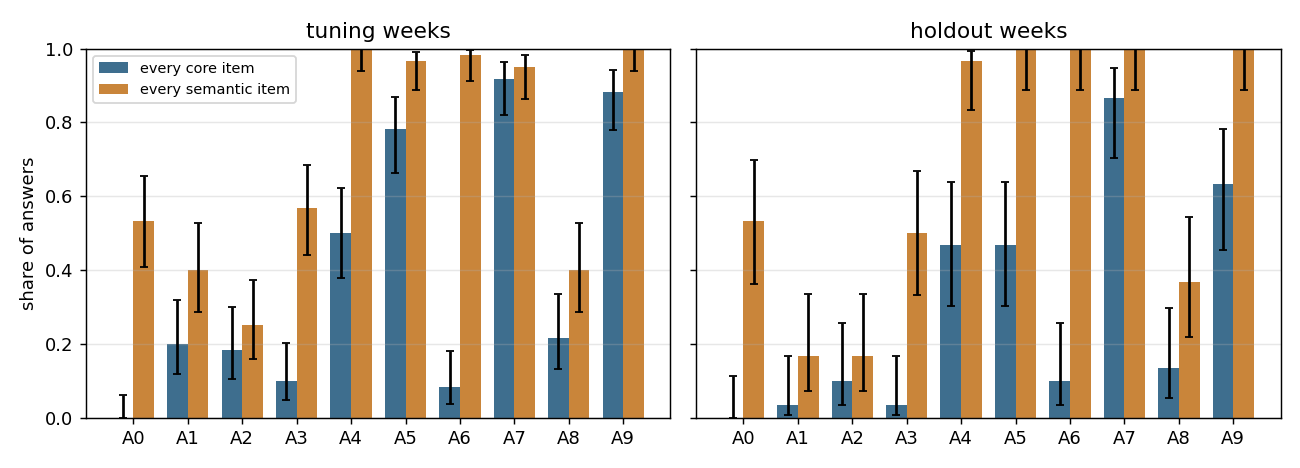
\includegraphics[width=\columnwidth]{figures/pass_rates.png}
\caption{Weekly review: share of answers passing every core item and every semantic item, with 95\% Wilson
intervals.}
\label{fig:weekly}
\end{figure}

Table~\ref{tab:weekly} and Figure~\ref{fig:weekly} separate the effects of the digits, the verdicts, the implications and the answer structure.

\paragraph{Verdicts reduce hallucination, not wrong advice (RQ1).} Replacing numbers with verbal verdicts (A1 to A2)
raised the pass rate of hallucination items from 73\% to 89\% on held-out weeks (80\% to 93\% on tuning weeks), and
the misread calorie comparison disappeared. The share of answers whose advice passed every semantic item did not
change (17\% to 17\%; paired difference in semantic items passed $+0.085$, 4 wins, 2 ties, 4 losses, $p=0.48$).

\paragraph{Digits or completeness? (ablation A8).} A2 changed two things at once: it removed the digits and it
stated the calorie verdict that the numeric block lacks. A8 separates them. It uses A1's prompts and checks, keeps the
whole numeric block and appends A2's verdict lines, so the model sees every figure and every verdict. A8 is
statistically indistinguishable from A1 (every core item passed: 13\% vs.\ 3\% of held-out and 22\% vs.\ 20\% of
tuning answers; held-out paired difference $+0.019$ in core items, 6/1/3, $p=0.26$) and from A2 in the share of core
items passed ($-0.008$, 3/1/6, $p=0.65$). Its hallucination items stay at 78\% on held-out weeks (77\% on tuning
weeks), against 89\% (93\%) for A2 and 73\% (80\%) for A1, and its observations still contain 19.7 digits on average.
Stating the missing verdict therefore did not reduce the factual errors; removing the digits did. Neither change made
the advice correct: 37\% (40\%) of A8 answers pass every semantic item, against 17\% (40\%) for A1.

\paragraph{Digits with the implications present (ablation A9).} A8 kept the digits but added only verdicts, which carry
no implications, priorities or plan. A9 asks the reverse question. It is A7 with the numeric block added under the
description, the ``no digits'' rules replaced by ``use a figure from the figures above exactly as given'', and the
no-digits answer check replaced by the figure check of the numeric designs; the description, the priorities, the kinds
of fix and the numbered plan are identical. Scored with the same frozen checklist, A9's advice is as good as A7's:
every semantic item passed in 100\% of held-out and tuning answers (A1: 17\% and 40\%). The invented figures come
back: 23\% of held-out answers (A7: 0\%, A1: 30\%) and 10\% of tuning answers (A7: 0\%, A1: 12\%) contain a figure that
is not in the data, so hallucination items pass 83\% against 100\%. Answers passing every core item were 63\%
[46--78] on held-out weeks (A7: 87\%, A1: 3\%) and 88\% on tuning weeks (A7: 92\%, A1: 20\%). On the 10 held-out weeks A9
against A7 is $-0.019$ core items per week (0 better, 6 tied, 4 worse, $p=0.125$), too few weeks to call, while A9
against A1 is $+0.091$ (10 better, $p=0.002$). A9 is also slower than A7 (6.3 against 5.2\,s) and redrafts more often
(50\% against 33\%). A figure that is in the data can still be used wrongly, and the checklist passes it: for a week
with an average of 96\,g of protein against a 180\,g target, one answer advised a dinner swap ``to boost intake by around
96\,g'' and a snack ``to add another 96\,g'', using the average as the amount to add, twice.
Two separate effects follow: code-supplied implications, priorities and plan make the advice correct and the format
right, with or without the digits, and the digits are what bring the factual errors back.

\paragraph{Implications fix the advice (RQ1).} Adding sizes, directions and a ``keep as is'' list (A3) raised the
semantic share to 50\%. It also lowered specificity from 92\% to 66\%, because the list came back as recommendations
to keep a metric as it is. Adding implications, admissible links, phase-weighted priorities and fix kinds (A4) raised
it to 97\% (tuning 100\%; paired $+0.117$, 7/3/0, $p=0.016$). A blind judge preferred A4 over A2 on substance in 10
of 10 held-out weeks (J3).

\paragraph{Structure drives format (RQ1).} With the plan written as a list of items, the model copied the list format
(``Recommendation one:''). Instruction items fell to 89\% and answers passing every item to 10\% (A5 to A6: $-0.056$,
1/0/9, $p=0.006$). Stating the same plan as one sentence restored the format (A7: 87\% of held-out answers pass
every item; A7 vs.\ A6 $+0.093$, 10/0/0, $p=0.002$). Against the numeric two-question design, A7 improved the
per-week share of core items passed in 10 of 10 held-out weeks ($+0.110$, $p=0.002$) and of semantic items in 9
($+0.358$, $p=0.004$).

\paragraph{Thinking mode.} The original single prompt in thinking mode (A0) passed every core item in no answer, at
39.6\,s per review. Its advice was more often correct than that of the fast numeric design (53\% vs.\ 17\% of answers
passing every semantic item; $p=0.008$), so reasoning recovers part of the missing implications, at five times the
latency and without fixing the format. Labels reached 100\% on the semantic items in non-thinking mode at 5.2\,s.
A0 also differs from A1 in using a single prompt, so this is not a clean ablation of thinking mode.

\subsection{Checkpoint comment and morning briefing}
\label{sec:res-messages}

\begin{table}[t]
\centering\small
\setlength{\tabcolsep}{3.2pt}
\begin{tabular}{@{}lrrrrr@{}}
\toprule
ID & Held-out [95\% CI] & Tuning & Incident & s & Redraft\\
\midrule
C0 numbers & 33\% [19--51] & 60\% & 14\% & 4.1 & 0\%\\
C1 labels v1 & 77\% [59--88] & 90\% & -- & 2.1 & 0\%\\
C2 \quad + checks & 87\% [70--95] & 88\% & 29\% & 2.0 & 0\%\\
C3 labels v2 & 77\% [59--88] & 90\% & -- & 2.2 & 0\%\\
C4 \quad + checks & 80\% [63--90] & 88\% & 43\% & 2.3 & 10\%\\
C5 labels v3 & 97\% [83--99] & 96\% & 100\% & 1.9 & 0\%\\
C6 \quad + checks & \textbf{100\%} [89--100] & 96\% & 100\% & 1.9 & 13\%\\
\midrule
B0 numbers & 37\% [22--54] & 65\% & 47\% & 3.3 & 0\%\\
B1 labels v1 & 53\% [36--70] & 68\% & 27\% & 4.0 & 0\%\\
B2 \quad + checks & 40\% [25--58] & 48\% & -- & 4.9 & 50\%\\
B3 labels v2 & 63\% [46--78] & 83\% & -- & 4.1 & 0\%\\
B4 \quad + checks & 60\% [42--75] & 82\% & -- & 4.1 & 3\%\\
B5 labels v3 & 83\% [66--93] & 78\% & 60\% & 3.6 & 0\%\\
B6 \quad + checks & 97\% [83--99] & 82\% & 73\% & 3.8 & 10\%\\
B7 labels v4 & 90\% [74--97] & 96\% & 80\% & 3.4 & 0\%\\
B8 \quad + checks & \textbf{100\%} [89--100] & 100\% & 100\% & 3.7 & 37\%\\
\bottomrule
\end{tabular}
\caption{Share of answers passing every applicable item of checklist v1.7 (30 held-out, 60 to 80 tuning and 21 or 15
incident answers per row), seconds per answer and redraft rate on held-out cases. The incident cases (7 checkpoints,
5 mornings) were written from the deployed message after the v1.5 rules existed; a dash marks a design not run on
them. Earlier versions of this table, scored with v1.4, showed C3/C4 at 100\% and B1 at 90\%. Rules added later lowered
the older designs: the end-of-day rule (v1.6) took the original checkpoint prompt from 53\% to 33\% held-out, because
all 18 of its last-check answers talk as if the day went on.}
\label{tab:messages}
\end{table}

\begin{figure}[t]
\centering
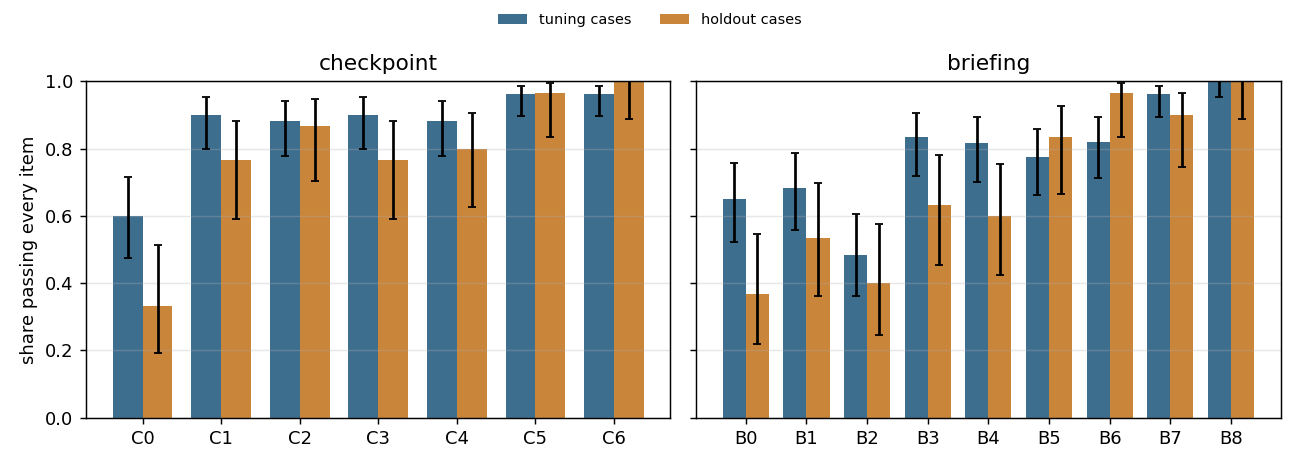
\includegraphics[width=\columnwidth]{figures/message_pass_rates.png}
\caption{Checkpoint comment and morning briefing: share of answers passing every applicable item, with 95\% Wilson
intervals.}
\label{fig:messages}
\end{figure}

\paragraph{Transfer (RQ2).} Labels removed the error classes of the numeric designs (Table~\ref{tab:messages},
Figure~\ref{fig:messages}). With the original checkpoint prompt, internal codes reached the user in 7\% of tuning and
20\% of held-out answers (``which is a status~3''); answers repeated the false budget statement (``200\,kcal over
your daily budget'' at 15:00 with 1{,}700 of 3{,}000\,kcal eaten); and one answer suggested ``a rice bowl or granola
bar for calories'' in a fat-loss phase that was already over plan. With the original briefing prompt, a training day
was called a rest day in 22\% of applicable tuning answers and 50\% of applicable held-out answers (17 answers across 9
cases), plausibly read from the numbered instruction ``a brief workout or rest day note''. None of these occurred
with labels. The checkpoint comment also became faster (4.1 to 2.0--2.3\,s) and shorter (112 to 58--65 words), with
a prompt about half the size (714 to 385--390 tokens).

Pooled over 30 cases, C6 improved on C0 in 17 cases, tied in 13 and lost none ($p<0.001$); B8 improved on B0 in 17,
tied in 13 and lost none ($p<0.001$). On the 10 held-out cases alone the paired differences are $p=0.008$ (C6 vs.\ C0)
and $p=0.016$ (B8 vs.\ B0). The failures are concentrated in a few situations, so per-case tests have little power;
the evidence is also which error classes disappear.

\paragraph{What labels break.} The model verbalizes what the view contains. With labels v1, the day's last check
repeated the daytime weather lines at 23:59 and exceeded its length limit. A 55\% gap was once softened to
``slightly over''. A plan saying ``the first thing to do better'' produced reflections that named one of two large
misses. Version~2 of the checkpoint removed the unneeded lines and, under checklist v1.4, passed every item in all 90
answers. Version~2 of the briefing improved the tuning set (90\% to 95\%) and degraded the held-out set (90\% to 77\%)
under v1.4. Asking
it to name every listed item produced six-sentence reflections on held-out mornings with four or five items, and its
example ``(such as a twenty-minute walk)'' came back as the movement suggestion, twice as an outdoor walk on a day with
unknown weather. The held-out set exposed both.

\paragraph{A message the checklist could not see.} The checkpoint comment of a deployed system (version~2, gain phase,
rain, a lower-body session already logged) read: ``focus on getting more movement in without going outside \ldots{}
You've got fish oil, chicken breast, and a protein shake \ldots{} Maybe do some light squats or lunges at home to add to
your steps.'' Checklist v1.4 passed it. The user's review named three errors that no item covered: exercises are not
steps, training comes from the user's plan, and the advice ignored the hour. The food list had also admitted a
supplement (45\,kcal, no protein) as a ``light option''. Checklist v1.5 adds the rules. Under it, 9 of 111 checkpoint
answers of version~2 name an exercise, 11 of 21 incident answers offer a supplement as food, and in the briefing 27
of 105 answers of version~1 name an exercise as the step idea (original prompts: 28 of 111 and 32 of 105). So the
defect was frequent, and the earlier results overstated version~1 and version~2. Version~3 states the missing
concepts. It names no exercise in any checkpoint answer (0 of 131) or checked briefing answer (0 of 112), passes all 21
checkpoint incident answers, and 11 of 15 briefing incident answers (three misses are the yesterday part leaving out a
second large miss; one is an outdoor walk that survived the redraft). Version~4 of the briefing removes the
omissions (below). Without checks, 7 of
112 briefing answers still name an exercise,
and on the unknown-weather incident case the unchecked briefing sent the user for a walk ``around the block'' in 3 of 3
answers; the checks removed both.

\paragraph{The yesterday part.} Version~3 of the briefing still failed on the yesterday reflection: 14 checked answers
named only the first of several large misses. Version~4 (above) passes every check in all 124 answers of the three case
sets, including 30 of 30 held-out and 15 of 15 incident answers; version~3 passed 97\% of the held-out answers once the
weigh-in rule was corrected, so on held-out cases the two are within noise (B8 vs.\ B6: 1 case better, 9 tied, none
worse, $p=1.0$), and the gain shows on the tuning and incident cases, which exposed the problem. The first run of
version~4 revealed a new failure on days with no misses: a closing ``Keep up the great work, G.'' used the name twice.
The first checks did not look for it; the prompt now stops after the last planned sentence and the checks look for a
repeated name and a closing pep line. At the day's last check the original prompts talked as if the day went on in all 18
answers (``on track'', ``next block'', ``keep going''), labels v1 in 1 of 18, v2 in 3 of 18 and v3 in none, which states
that the day is over.

\subsection{Answer checks}
\label{sec:res-checks}

Once the representation was right, answer checks added little (RQ2). For the checkpoint, checked and unchecked
designs differed in at most two cases per set; the only visible effect was the removal of the softened gap. For the
briefing, the version-1 checks redrafted 50\% of briefings, nearly all for a duration such as ``a 20-minute walk''.
The labels prompt forbade such durations, while the product rule allows them. Under v1.4 the checks changed no held-out outcome
(90\% vs.\ 90\%) and added about one second. A first, keyword-based outdoor check also fired on mentions and rewrote
correct answers. The first checklist, which used the same naive rule, rewarded the rewrites, an apparent gain that
vanished when both were corrected and the affected configurations were run again. With version~3 the checks
mattered for the briefing: 83\% of held-out answers passed without them and 97\% with them (version~4: 90\% and 100\%),
and 60\% against 73\% (version~4: 80\% against 100\%) on the incident cases, mainly because they stopped the outdoor walk
on unknown-weather days and the closing sign-off, at about 0.2\,s per answer on average and with 10--37\% of answers
redrafted. For the checkpoint the checks moved
97\% to 100\%.

\subsection{Other models (RQ3)}
\label{sec:res-models}

The labels were written and tuned on qwen3:8b only. We repeated the key comparisons on three other model families served
by Ollama in the same 4-bit format (llama3.1:8b, gemma3:4b, mistral:7b), with the same cases, three runs each and the same
frozen checklists, each model in its own folder so that no run can mix into another. Table~\ref{tab:models} shows the share
of held-out answers that passed every item. The label designs improved the paired per-case score significantly (Wilcoxon,
$p<0.001$) in eight of the nine model--message comparisons. The exception was gemma3:4b on the briefing ($-0.04$,
$p=0.71$; 47\% against 37\%). The size of the gain varied with the model. llama3.1:8b reached 90--93\% on all three
messages. mistral:7b could not meet the weekly review's format under either representation (0\% of answers passed every
item), yet words still won 28 of 30 cases on the finer per-case score ($+0.09$). A fifth model, olmo-3:7b, was dropped:
it is a thinking model and one weekly case took 22 minutes, so the full run would have taken about 33 hours.

\begin{table*}[t]
\centering\small
\caption{Held-out answers passing every checklist item (\%; $n=30$ per cell, three runs of 10 cases). Numbers = original
prompt; words = the label design (weekly A7, checkpoint C6 with checks, briefing B8 with checks).}
\label{tab:models}
\begin{tabular}{lrrrrrr}
\toprule
 & \multicolumn{2}{c}{Weekly review} & \multicolumn{2}{c}{Checkpoint} & \multicolumn{2}{c}{Briefing}\\
Model & numbers & words & numbers & words & numbers & words\\
\midrule
qwen3:8b & 3 & 87 & 33 & 100 & 37 & 100\\
llama3.1:8b & 3 & 90 & 30 & 93 & 13 & 93\\
gemma3:4b & 3 & 70 & 17 & 87 & 37 & 47\\
mistral:7b & 0 & 0 & 33 & 100 & 0 & 40\\
\bottomrule
\end{tabular}
\end{table*}

\subsection{A fourth surface: the conversational agent (RQ3)}
\label{sec:res-chat}

The app also has a free-text chat agent. In its original design it received raw figures through three tools, answered many
questions with a canned dump of the calorie log or the step table, and did its own arithmetic. A first check on one real
evening found it answering ``how am I doing today'' with 983 kcal remaining when the day was 10 kcal over, and computing
``1,950 $-$ 263 = 1,687 remaining'' for a pizza it had invented a calorie figure for. We built the words design
(\texttt{chat\_facts.py}): code states where calories, protein and steps stand against the plan for this hour, an overall
verdict, what the phase's goal means for the day, how much of the day is left and what still fits the hour, and judges a
size in the question (``is 500 kcal too much'') against what is left. Exact figures appear only when the question asks for
one. The model has no tools, and its answer is checked (figures not in the facts, exercises, invented workouts, shouting,
claims of having logged, advice that works against the phase) and redrafted at most twice. The original design is kept
runnable behind a switch. Both run through the real agent graph on made-up days; every route to the live database is cut.

Each case is one fake day and one question. We tuned on 20 cases, then evaluated on sets that no design decision had seen:
a first held-out set of 10 cases (three runs), then, after its failures had been read and fixed, a fresh set of 16 and,
after that, another fresh set of 20, each run once with the design and checklist frozen. Table~\ref{tab:chat} shows the
results. On the fresh sets the words design passed 92\% (44 of 48) and 90\% (54 of 60) of answers against 21\% and 15\%
for the original; in 34 and 45 pairs only the words design passed and in none did only the original ($p<10^{-9}$, exact sign
test). On the first held-out set it was 80\% against 27\% (18 pairs against 2, $p=0.0004$). The original design also
produced failures that only reading revealed: it invented a bodyweight circuit (jump squats, planks) in all three runs of
``give me a quick workout'', and in two answers it printed its internal context block to the user. Answer checks added
two passes on one fresh set and nothing on the others. Each set's remaining misses were fixed only before the next
fresh set: a count several hours old that was not mentioned, a status answer that left out part of the day, and a narrated
``based on the facts''. The last of these still failed in all three runs of the final set.

Two things limit the claim. The checklist was edited after the first held-out set (version 1.4), because it flagged
figures that the original design prints from the system (a step-discount note, a negative protein remainder, the food
list's calories); the edit only removes false flags from the original design, but it was made after a result was seen.
And the chat comparison on other models (Table~\ref{tab:chat}) used all 66 cases once, including the 20 tuning cases, with the
original design on the fast backend for every model but qwen3, because only the qwen3 family accepts thinking mode in
Ollama, and gemma3:4b has no tool support, so 42 of its 66 original-design answers were API errors and not verdicts. The
words design was ahead on every model: by 69--80 points on three, and by 27 points on mistral:7b, where its answers were too long
for the length rule (41\% against 14\%).

\begin{table}[t]
\centering\small
\caption{Chat agent, 66 fake-day cases, one run each: answers passing every checklist item. $^\dagger$42 of 66 original-design
answers were API errors (no tool support).}
\label{tab:chat}
\begin{tabular}{lrrr}
\toprule
Model & original & words & only words / only orig.\\
\midrule
qwen3:8b & 15 & 95 & 53 / 0\\
llama3.1:8b & 20 & 89 & 47 / 1\\
gemma3:4b$^\dagger$ & 12 & 85 & 50 / 2\\
mistral:7b & 14 & 41 & 23 / 5\\
\bottomrule
\end{tabular}
\end{table}

\paragraph{After these sets.} A user's own review of a real conversation found two more errors that no set had
covered: asked about the workout of the day, the chat advised ``rest and recover properly today'' on a training day, and
it described an upper-body day as back, chest and arms with a muscle-building focus that the plan never stated. We
added the training week, the muscles each day's exercises train and the user's injuries to the facts, and two answer checks
(advice to rest that the facts do not give; a muscle or a muscle-building focus the facts never gave the workout).
The checklist is now version~1.11. This version was not evaluated on a fresh set, so none of the chat figures above
describe it, and the raters below saw the design as of 5~October.

\subsection{Human ratings (RQ4)}
\label{sec:res-human}

Six people compared the two designs blind. Each saw the same synthetic day and two messages in random order, and
chose the one they would rather receive (\emph{overall}) and the one that was more accurate about the data shown
(\emph{accuracy}), with ``equal'' and ``both poor'' allowed. The first kit had 36 items and was rated by one person;
the second had 22 items and was rated by five. Four of the six describe themselves as professionals in fitness or
nutrition and two as having some background. A few items were shown twice with the sides swapped, to check that a rater
was consistent. The answer key of the first kit was overwritten after it was sent and was rebuilt from the saved page
and the saved evaluation answers; every item matched one answer, and the rebuilt key reproduces the earlier tally.
Table~\ref{tab:human} counts only items where a rater chose a side.

\begin{table}[t]
\centering\small
\caption{Blind comparison, words design against the original prompt, six raters pooled. Items per rater are not
independent, so the intervals are optimistic.}
\label{tab:human}
\begin{tabular}{@{}lrrrr@{}}
\toprule
& words & original & share & 95\% CI\\
\midrule
\multicolumn{5}{@{}l}{\emph{Which would you rather receive?}}\\
Weekly review & 17 & 7 & 71\% & 51--85\\
Checkpoint & 13 & 12 & 52\% & 33--70\\
Briefing & 11 & 9 & 55\% & 34--74\\
Chat & 11 & 13 & 46\% & 28--65\\
All four & 52 & 41 & 56\% & 46--66\\
\midrule
\multicolumn{5}{@{}l}{\emph{Which is more accurate?}}\\
Weekly review & 11 & 11 & 50\% & 31--69\\
Checkpoint & 10 & 11 & 48\% & 28--68\\
Briefing & 7 & 5 & 58\% & 32--81\\
Chat & 8 & 11 & 42\% & 23--64\\
All four & 36 & 38 & 49\% & 38--60\\
\bottomrule
\end{tabular}
\end{table}

The result is not a preference for the label design. Only the weekly review is above 50\% with an interval that stays
above it; the chat leans to the original, and the interval over all four types includes 50\%. On accuracy, raters most
often chose ``equal'' or split evenly, so they did not see the difference the checklists count: the share of
answers with a wrong figure is a property a reader notices only when the figure is plainly wrong, and a person who sees
one version cannot compare it. Agreement between raters was close to zero (Krippendorff's $\alpha$ from $-0.14$ to
$0.05$ per kit and message type for the overall question). On the repeated items, one rater chose the same side
in 1 of 4 judgments and another in 4 of 12, while three were fully consistent, so the spread between people is larger
than the difference between designs. Four of the six raters left comments. They asked for shorter messages, a positive tone that does not over-analyse small misses (one professional
called results within 5\% of target highly consistent), the context of the client's day before advice, and food advice
that matches the missing nutrient. One rater independently noted the numeric errors of the original prompts that the
paper counts, a total of 3{,}900 called under a target of 3{,}000 among them. Raters who preferred the original named
style or completeness and not accuracy. These are six volunteers, the items are synthetic, and the checklist that
selected the designs was written by us. The study was not designed to show that the label messages are no worse, and we
read the table only as: no clear preference was found, with a lead on the weekly review and a lean the other way on the chat.

% ─────────────────────────────────────────────────────────────────────────────
\section{Discussion}
\label{sec:discussion}

\paragraph{Why numeric prompts fail here.} We observe four mechanisms.
\emph{Offloaded comparisons.} The numeric prompts left a third (weekly), 58\% (checkpoint) and 29\% (briefing) of the
needed verdicts implicit. In non-thinking mode, single-pass generation has to compute each implicit comparison
while decoding the sentence that states it, and the calorie sign error occurred on the one weekly metric without a
precomputed verdict. Prior work links such failures to how numbers are segmented and represented
\citep{nogueira2021investigating,singh2024tokenization,thawani2021representing}. We did not isolate tokenizer or
quantization effects; cl100k\_base counts in this paper are a length proxy only.
\emph{Multi-step implications.} Moving from a verdict to advice takes several steps: comparison, direction,
phase-dependent valence (under-eating is acceptable in a fat-loss phase and a problem in a gain phase), priority and
kind of fix. Verdicts supply the first step; the advice became correct only when code supplied the remaining steps
(17\% to 97\%). Putting the figures back next to those steps (A9) left the advice correct and brought back invented
figures, so the two effects separate: the implications and the plan make the advice right, the digits are the source of
the factual errors. Thinking mode recovered part of this chain (53\%) at five times the latency.
\emph{Prompt defects.} The baseline checkpoint prompt contained statements false as worded, and the model repeated
them. Verdict coverage and a truth audit of the prompt locate such defects without running a model.
\emph{Copying.} The model realizes what its context contains: instruction lists, numbered topics, internal codes,
lines the message does not need and examples. Up to 14\% of the word 4-grams in label-based answers were copied
verbatim from the view. This is a generation-side counterpart of distraction by irrelevant context
\citep{shi2023distracted}.

\paragraph{Design rules.}
\begin{enumerate}[label=R\arabic*.]
\item State every comparison the message depends on as a verdict, and measure verdict coverage.
\item State implications for the goal, the priority order and the kind of fix, not only positions.
\item Give each question only the view it needs; remove lines the message must not mention.
\item State the answer plan as one sentence; avoid numbered instruction lists and examples that can be copied.
\item Pass no internal codes, and audit every prompt statement for truth.
\item Validate answer checks and checklists by reading what they flag, and ablate the checks.
\item Accept a revision only if it holds on held-out cases.
\item State the domain concepts the model cannot know (what a step is, where training comes from, which weather sends
activity indoors, what the hour allows) in the view, write a checklist item for each, and have a domain user read real
messages: recall is not measured by a checklist its authors wrote.
\item When the answer must cover a list, let code rank it, count it and fix the sentence budget; an instruction such as
``the first thing'' or ``every item'' leaves the model to choose the length and loses items.
\end{enumerate}

\paragraph{Cost.} Labels lengthened some prompts but reduced latency through shorter answers and fewer redrafts:
7.4 to 5.2\,s for the weekly review and about 4 to 2\,s for the checkpoint. The briefing became 0.7--0.8\,s slower;
its answers were about 20 words longer.

% ─────────────────────────────────────────────────────────────────────────────
\section{Limitations}
\label{sec:limitations}

The cases are synthetic, 30 per message type, and target known failure modes, so failure rates are higher than in
ordinary use. The main evaluation uses one model in one quantization format, at one temperature, in one domain; three other model
families (Section~\ref{sec:res-models}) used the same cases and checklists, but the labels were written for qwen3:8b only, and one of
them could not meet the weekly format under either representation. The chat-agent sets were evaluated one after another
and each became tuning data once its failures were read, and the checklist was edited once after a result was seen. The checklists
were written by the same party that designed the labels, from the same product rules. Their precision was measured
by reading flags, but recall was not measured, and a deployed message showed a failure that checklist v1.4 missed. Its
replacement, v1.5, was written after that message and version~3 was designed against it, so the incident-set scores of
version~3 are partly by construction; the tuning and held-out cases predate the rules. The secondary judge is an LLM of the same family as the assistant that
built the configurations. The human evaluation has six volunteers, two kits with different items, a rebuilt answer
key for the first kit and a chat design that has since changed, and its raters hardly agree; it found no clear
preference either way and is too small to test non-inferiority. Per-case paired tests have little power at $n=10$--$20$.
The version-2 revisions for the checkpoint and briefing each answer failures seen on tuning cases, but the same failures
had also been seen on held-out cases while the checklist was being validated, so the version-2 held-out results are
less clean than those of version 1. Thinking mode was tested only in the original single-prompt design. We ran no program-aided or tool-using baseline
\citep{gao2023pal,schick2023toolformer}, in which the model would compute the verdicts itself with code. The A8 and A9
ablations were run on the weekly review only; the checkpoint and briefing have no digits ablation. A9 is one design
with one extra answer check (the figure check of the numeric designs) and was scored with the frozen checklist, whose
figure item cannot see a true figure used in the wrong role. Token
counts use a proxy tokenizer.

\section{Ethics and Participant Protection}

The evaluation used synthetic fitness-coaching cases and did not involve real user health records or medical
interventions. Six adult volunteers located in Guatemala, Belgium, and the United States participated in a research
evaluation of AI-generated messages. Participants were informed of the research purpose and participated voluntarily.
Ratings are reported only in aggregate, without participant identifiers. The study was conducted independently without
institutional sponsorship, supervision, funding, or resources. No institutional ethics review was sought or obtained.

\paragraph{Broader impact.} The messages give fitness and nutrition suggestions against targets that users set
themselves, and they are not medical advice. Running the model locally keeps personal health data on the user's device.
Advice errors in this domain can encourage under-eating or overtraining.
The checklist therefore includes rules against recommending extra movement to a user who under-ate and against
asking a user in a fat-loss phase to catch up on calories, and production keeps deterministic fallbacks when the
labels path fails.

\section{Conclusion}

For a 4-bit 8B model writing data-grounded coaching messages, the representation of the input mattered more than the
reasoning mode. Turning numbers into verbal verdicts removed factual errors, and adding the figures back to the full design brought
them back. Stating implications, priorities and
fix kinds in code made the advice correct, and shaping the prompt as one view per question with a one-sentence plan
fixed the format. The model copied whatever the view contained, so the view must hold exactly what the message needs,
and every revision should be judged on held-out cases. The same held for a conversational agent and across three further
model families, with one clear exception and a smaller gain on the weakest model. A small blind human comparison did
not find a clear preference (56\% of decisive choices for the label messages, interval 46--66\%), with a lead on the
weekly review and a lean the other way on the chat. The accuracy gains that the checklists count were not visible to
these raters.

The deployed system has since gained a knowledge layer that matches exercise names to muscles and states what a
training focus, a phase and an injury mean for the day. It uses the same principle: code decides, the model words it.
It is not evaluated here, and we leave it to later work.

\section*{Code and Data Availability}
The code, the synthetic cases (90 for the weekly review, checkpoint comment and briefing, 66 for the chat), all saved
answers, the checklists and the report generator are available at
\url{https://github.com/GGHOSTRADER/implications-not-just-words}. The code is under the PolyForm Noncommercial License
1.0.0; the cases, answers and report are under CC BY 4.0. The repository recomputes every table from the saved answers
and checks, through the stored version fingerprints, that its code is the code that produced them. The weekly, checkpoint
and briefing answers can be regenerated with a local Ollama, and a small chat agent reruns the chat design. The
application's own chat agent, which produced the saved chat answers, and the human ratings are not released; only the
counts in Table~\ref{tab:human} are.

\section*{Use of AI Assistance}
An AI assistant (Claude, Anthropic) helped write the labelers, the checklists, the analysis code and the text of this
paper, and the secondary judge in the blind judgments (Section~\ref{sec:limitations}) is a model of the same family. The
author is responsible for the content; the numbers come from the generated report.

\bibliographystyle{plainnat}
\bibliography{references}

% ─────────────────────────────────────────────────────────────────────────────
\appendix
\onecolumn
\section{Checklist Items}
\label{app:items}

\paragraph{Weekly review, core rubric v2.1 (22 items).}
\emph{Hallucination:} no invented numbers (every figure about the week matches the data within 2\%; proposals such
as ``20 minutes'' allowed in recommendations); no recommendation moves a metric the wrong way; no metric without data
is described.
\emph{Instruction:} exactly two paragraphs; no markdown; no label or heading; no greeting; no sign-off; each paragraph
150--700 characters; no advice wording in the observations; one to three recommendations numbered from 1.
\emph{Coverage:} the observations discuss every metric with data; every off-target metric is named in the
recommendations.
\emph{Specificity:} each recommendation names an amount, time, place or habit; no filler phrases; no recommendation
slot spent only on keeping something as it is.
\emph{Semantic:} each problem gets an action of the matching kind; recommendation 1 addresses a problem when one
exists; a calorie gap of 15\% or more is addressed first with a food change; no added movement before a food change
when calories are under target; no connection claimed that the data cannot support; each stated consequence is
attached to the metric it belongs to.

\paragraph{Checkpoint comment, message checklist v1.7 (21 items).}
\emph{Hallucination:} figures match the data (within 2\%, proposals allowed); never says the daily budget is exceeded
while the day's total is under target; a calorie sentence never states the opposite position; a gap of 30\% or more
is never called slight, and one under 10\% never called far; no request for more food while over plan, no catch-up
in a fat-loss phase, no request for less food while under plan outside a fat-loss phase, no request for more protein
once the day's protein is met.
\emph{Instruction:} no greeting or sign-off; no headings or lists; two to nine sentences (two to five at the last
check); never treats the closed block as still running.
\emph{Semantic:} the last check gives no advice for a next meal or tonight; no outdoor movement suggestion when
outdoor walking is unsuitable or unknown (conditional suggestions allowed when unknown); with nothing logged, no
scolding and a nudge to log or eat; no disliked food; no energy-dense food while over plan and a protein food when
protein is behind; every metric off plan in a way that matters for the phase is mentioned; no internal codes.
\emph{Added in v1.5:} no exercise is named (squats, lunges, circuits, yoga, sets, reps); no extra, additional or
different workout, and none at all after a session is logged or on a rest day; no breakfast from 11:00, lunch from
15:00 or dinner and snacks from 22:00, and no walking idea from 22:00; a supplement in the food list (fish oil,
creatine, vitamins) is not offered as food. The weather item also treats great heat (32\,\textdegree{}C and above) and
strong wind (40\,km/h and above) as reasons for indoor steps, allowing an outdoor walk only next to an indoor
alternative. \emph{Added in v1.6:} the day's last check does not talk as if the day went on (no ``on track'', ``still
time'', ``keep going'', ``catch up'', ``tomorrow'').

\paragraph{Morning briefing, message checklist v1.7 (19 items).}
\emph{Yesterday:} a greeting with the user's name exactly once; two to five sentences; no repeated figures; no list or
sign-off; no praise for a metric that was off and no metric that was met called short; no praise for an unlogged
workout or weigh-in; every miss of 10\% or more is mentioned.
\emph{Today:} no greeting or name; two to four sentences; no figures except the temperature and proposals; no list
or sign-off; a training day is never called a rest day; a food idea, a movement idea and a workout note; the outdoor
rule; when today's calorie target changed, no statement of the opposite direction; a lowered target gets no hearty
breakfast and a raised one is not told to eat less; on a rest day, no push to train. \emph{Added in v1.5:} no exercise
is named; no extra or additional workout, and none on a rest day. \emph{Corrected in v1.7:} praise for the weigh-in is read
per sentence, and a sentence that looks forward (``don't forget to get your weigh-in done'') is advice, not praise.

\section{Reproduction}
\label{app:repro}
Answers: \texttt{python -m evals.run\_weekly\_eval} (weekly review) and \texttt{python -m evals.run\_message\_eval}
(checkpoint, briefing), each with \texttt{--set tuning|holdout --repeats 3}. Representation measures:
\texttt{python -m evals.label\_metrics} and \texttt{python -m evals.message\_metrics}. Report with every table above,
recomputed from the saved answers: \texttt{python -m evals.report}. Checklist validation samples:
\texttt{python -m evals.validate\_rubric} and \texttt{python -m evals.validate\_message\_rubric}. Fingerprints of
every configuration and the result files used are listed in the generated report.

\end{document}
